%\documentclass[twoside,openright,a4paper,11pt]{book}
%
%
\usepackage[utf8]{inputenc}
\usepackage[francais]{babel}
\usepackage[T1]{fontenc}

\addto\captionsfrench{\def\tablename{\textsc{Tableau}}}% pour avoir TABLEAU et pas TABLE dans les légendes des tableaux

%%%%%%% MISE EN PAGES %%%%%%
\usepackage{geometry}
\geometry{outer=2cm,inner=3cm,top=3cm}

\setcounter{tocdepth}{3}     % Dans la table des matieres
\setcounter{secnumdepth}{3}  % Avec un numero.
\usepackage{setspace}

\usepackage{fancyhdr}	% marge en haut et en bas
\pagestyle{fancy}

\fancyhead{}	% vide l'entête
\fancyfoot{} % vide le pied~de~page

\fancyhead[RO]{\leftmark}
\fancyhead[LE]{\rightmark}
\fancyfoot[C]{\thepage}	% numéro de page en bas au centre

\renewcommand{\headrulewidth}{0.4pt} % épaisseur du trait en haut
\renewcommand{\footrulewidth}{0.4pt} % épaisseur du trait en bas

\fancypagestyle{mypagestyle}{%
    \fancyhead{}	
    \fancyfoot{} 
    \fancyfoot[C]{\thepage}
    \renewcommand{\headrulewidth}{0.4pt} 
	\renewcommand{\footrulewidth}{0.4pt} 
}

\fancypagestyle{couvertureAbstract}{%
    \fancyhead{}	
    \fancyfoot{} 
    \fancyfoot[C]{}
	\renewcommand{\headrulewidth}{0pt} 
	\renewcommand{\footrulewidth}{0pt} 
}
%
\usepackage{layout}
\usepackage{tocbibind} % include tableofcontent in itself

%%%%%% PAGE DE GARDE %%%%%%

\geometry{outer=2cm,inner=3cm,top=3cm}
\usepackage[scaled]{helvet} % font used on cover (Helvetica)
\usepackage{eso-pic} % to set background picture
\usepackage{multicol} % for back cover (abstracts)
\usepackage{graphicx} % to include logos
\usepackage{tikz} % to compose background picture

% Colors (extracted from SPI's template)
\definecolor{boxcolor1}{rgb}{0.91373,0.92941,0.87451}
\definecolor{boxcolor2}{rgb}{0.94902,0.93333,0.91373}
\definecolor{boxcolor3}{rgb}{0.76078,0.87843,0.17647}
\definecolor{headercolor}{rgb}{0.94118,0.30980,0.17255}
\definecolor{namecolor}{rgb}{1.0,0.4,0.0}
\definecolor{titlecolor}{rgb}{0.19216,0.51765,0.60784}
% Also used: gray, teal (predefined by xcolor package, usually loaded by document class)

% Cover environment, to keep changes local
\newenvironment{cover}{%
  \fontfamily{phv}\selectfont % Select Helvetica font
  \pagestyle{empty} % No page number
}{
  \addtocounter{page}{-1}
  \cleardoublepage
}

% Macro for background common to front and back
\newcommand{\tikzBG}{%
  \path (0,0) rectangle (1,1);
  %TODO: You should adjust the bottom height of the following rectangle to fit your abstract's length
  \path [fill=boxcolor1] (.0571,.11) rectangle (.481,.963); 
  \path [fill=boxcolor2] (.4333,.697) rectangle (.9048,.7475);
  \path [fill=boxcolor2] (.4333,.7811) rectangle (.9048,.8316);
  \path [fill=boxcolor2] (.4333,.8687) rectangle (.9048,.9192);
  \path [fill=boxcolor3] (.0571,.7879) rectangle (.5762,.8316);
  \node[inner sep=0pt] at (0.2285,0.8788) [above left] {%
    
\includegraphics[height=.0707\paperheight,keepaspectratio]{./figures/logo/logo_unb.png}};
  \node[inner sep=0pt] at (0.6667,0.8788) [above right] {%
    
\includegraphics[height=.0808\paperheight,keepaspectratio]{./figures/logo/logo_ecn_color.png}};
  \node at (.0571,.8316) [above right,color=headercolor] {%
    \fontsize{29}{35}\selectfont\bfseries Th\`ese de Doctorat};
}

% Macro for repeated information (to avoid insconsistency)
%TODO: fill in with no formatting but desired case
\newcommand{\firstName}{Jean-Rémy}
\newcommand{\surname}{Gloaguen}
\newcommand{\thesisTitle}{Estimation du niveau sonore de sources d'intérêts au sein de mixtures sonores urbaines : application au trafic routier}

%%%%%%% SYMBOLES %%%%%
\usepackage{tipa}	% pour avoir l'accent concave
\usepackage{lmodern}	% pour les guillemets
\usepackage{gensymb}	% pour les degrés
\usepackage{enumitem}	% pour changer le symbole de l'item (\begin{itemize}[label=$\bullet$])

%%%%%%% EQUATION %%%%%%
\usepackage{amssymb}
\usepackage{amsmath}
\usepackage{fancybox}
\usepackage{xfrac}	% fraction de type "1/4"
\usepackage{cases}	% système équation
\usepackage[overload]{empheq}
\usepackage{bm}		% pour mettre en gras .
\usepackage{units} 	% x/y barre latérale pour les fractions
%
%%%%%%% FIGURE %%%%%%
\usepackage{subfigure}	% utiliser subfigure
\usepackage{float}	% utiliser H dans les figures
%
%%%%%% TABLEAUX %%%%%%
\usepackage{array,multirow,makecell}
%\addto\captionsfrench{\def\tablename{\textsc{Tableau}}}% pour avoir TABLEAU et pas TABLE dans les légendes des tableaux
\usepackage{colortbl} % pour avoir des lignes colorées dans les tableau
%\usepackage{slashbox} % pour les \backslashbox
%\usepackage{subcaption}
\usepackage{hhline}	% pour les lignes horizontales 
\usepackage{tabularx} % permet itemize dans les cellules
\usepackage{booktabs}
\usepackage{longtable}	% pour les tableaux longs

\newcolumntype{L}[1]{>{\raggedright\let\newline\\\arraybackslash\hspace{0pt}}m{#1}}
\newcolumntype{C}[1]{>{\centering\let\newline\\\arraybackslash\hspace{0pt}}m{#1}}
\newcolumntype{R}[1]{>{\raggedleft\let\newline\\\arraybackslash\hspace{0pt}}m{#1}}

%%%%% ALGORITHME %%%%%
\usepackage{algorithm}
\usepackage{algorithmic}

%%%%% BIBLIO %%%%%
\usepackage[fixlanguage]{babelbib}
\selectbiblanguage{french}
\usepackage{breakcites}	% pour couper les références en bout de ligne

%%%%% APPENDICES %%%%%%%
\usepackage[toc,page]{appendix}

%%%%%%%%%%%%%%%%%%%%%
\usepackage{url}	% gérer les adresses www.
\linespread{1.2}	% interligne

\cleardoublepage
%
%\begin{document}
%\newpage

\chapter{Méthode de séparation des sources sonores}


Savoir isoler les différentes composantes qui constituent un signal est une question complexe intervenant dans des domaines variés comme en biologie \cite{chiappetta2004blind}, dans le monde médical \cite{jung2000removing} ou bien encore dans le domaine de l'image \cite{} MISSING. En audio, cette question intervient alors que la quasi-totalité des environnements sonores qui nous entourent sont composées d'une multitude de sources sonores. En considérant, $N$ sources sonores, pour 1 capteur $i$, le problème de la séparation de source peut se poser comme un problème linéaire inverse :

\begin{equation}\label{eq:BSS}
x_i(t) = \sum_{j = 1}^{N}\sum_{\tau = 0}^{+\infty} a_{ij}(\tau)s_j(t-\tau)
\end{equation}

où $x_i(t)$ est un signal capté à l'instant $t$ au point $i$, $s_j(t)$ une source originale $j$ émise à l'instant $t$ et $a_{ij}$, le filtrage mixant de la source $j$ au point $i$. Une seconde approche similaire au problème \ref{eq:BSS} a également été proposée dans \cite{cardoso_blind_1998} :

\begin{equation}
x_i(t) = \sum_{n = 1}^{N}c_n(t)
\end{equation}

qui exprime le signal capté par le microphone $i$ comme la contribution de chacune des sources $n$ modulé par l'environnement. $c_j(t)$, appelé \textit{image spatiale de la source $n$}, s'exprime sous la forme $c_n(t) = (a_{ij} \ast s_j)(t)$.
Chacune source $s_j$ possède ses propres caractéristiques acoustiques (intensité, durée, fréquences), peut être émise simultanément avec les autres sources ou bien avoir entre elles des liens de causes à effets.
L'intérêt de développer des outils de séparation de sources sur de telles mixtures donne la possibilité d'éditer, d'analyser ou de modifier les composantes. Ceci est utile pour des applications comme par exemple,

\begin{itemize}
\item le débruitage de la voix pour améliorer la qualité des appareils auditifs,
\item l'amélioration de la reconnaissance de la voix dans des contenus audio-visuels,
\item la transcription des mélodies d'un morceau de musique,
\item la restauration de vieux enregistrements
\item \dots
\end{itemize}

De part la variété des sons, c'est donc une tâche complexe qui est à l'étude depuis plus de 30 ans. De ces recherches, plusieurs méthodes ont émergées qui diffèrent selon les applications visées. On propose dans ce chapitre de présenter certaines des méthodes les plus couramment utilisées pour déterminer celle qui est la plus adaptée a notre cas d'étude.

\section{Analyse de Scènes Auditives Computationnelle}

L'Analyse de Scènes Audio Computationnelle (abrégé CASA pour \textit{Computational Auditory Scene Analysis} en anglais) est une des premières techniques numériques cherchant à séparer les différentes sources composant un signal. Elle fut proposée par Brown \cite{brown1994computational} et se base sur la simulation de la réponse auditive humaine.
La méthode CASA est inspirée de l'Analyse de Scènes Auditives selon Bregman \cite{bregman1994auditory} qui explore les façons dont le cerveau humain comprend et organise les sons qui l'entourent. L'architecture de la CASA se décompose en 4 parties \cite{wang2006computational} :

\begin{itemize}
\item un filtrage cochléaire qui consiste en une suite de filtres passe-bas qui modélisent l'oreille externe et moyenne, et d'un filtre gammatone qui simule les réponses impulsionnelles de chaque cellule ciliée. Le signal obtenu est exprimé, en sortie, au travers d'un cochléogramme.
\item Une analyse temps-fréquence qui permet, au travers différents outils, d'augmenter les dimensions du problème et de mettre en évidence la présence de sons harmoniques notamment :
\begin{itemize}[label=$\bullet$]
\item la corrélation croisée entre les canaux fréquentiels proches pour faire émerger la présence des formants,
\item la corrélation croisée entre les deux canaux des deux oreilles pour localiser la source grâce à leur déphasage,
\item la fonction d'autocorrélation dans chaque canal pour faire émerger des maximas à des positions correspondant au période d'un son,
\item un lissage temporel afin de faire apparaitre des phénomènes de modulation,
\item \dots
\end{itemize}
\item Un groupement de sources qui consiste à ré-organiser les objets élémentaires pour construire les sources sonores en appliquant, par exemple, une contrainte temporelle  sur les représentations spectrales. Ce groupement peut se faire à partir du stimuli (CASA de type \textit{bottom-up}) ou bien à l'aide de schéma déjà établi (CASA de type \textit{top-down})
\item Un masquage binaire temps-fréquence est enfin construit pour chaque source identifié et est appliqué sur le spectrogramme initial permettant d'isoler les différentes sources sonores.\\
\end{itemize}

Développée à partir de la compréhension de certains aspects des capacités d'analyse des sons par notre cerveau, la méthode CASA a notamment trouvé des applications dans le domaine de la parole \cite{ellis1999using, brown2005separation, shao2010computational}. Des applications dans la reconnaissance de scènes sonores existent \cite{peltonen2002computational}. % mais les applications de cette méthode à ce genre d'environnement sont peu nombreuses.

\section{Algorithme DUET}

L'algorithme de séparation de sources DUET (\textit{Degenerate Unmixing Estimation Techniques)} est une méthode proposée par \cite{rickard2007duet} qui permet de déterminer $N$ sources sonores d'une mixture sonore à partir du déphasage et de l'atténuation entre les enregistrements de deux microphones $x_1(t)$ et $x_2(t)$. Cette approche se base sur 2 hypothèses : les signaux sont émis dans des conditions anéchoïques et il n'y a pas (ou très peu) de recouvrement fréquentiel entre les $N$ sources sonores $s_j(t)$. La condition d'anéchoïcité permet d'exprimer les 2 signaux captés sous la forme d'un signal exprimé en champ direct, $x_1(t) = \sum_{j = 1}^{N}s_j(t)$, et d'un autre déphasé, $x_2(t) = \sum_{j = 1}^{N} a_j s_j(t-\delta_j)$, pondéré par l'atténuation $a_j$ et en déphasage (positif ou négatif) $\delta_j$ avec la condition $\delta_j \leqslant \frac{d_{\mu_1,\mu_2}}{c_0}$ où $d_{\mu_1,\mu_2}$ est la distance entre les 2 microphones et $c_0$ la célérité du son. En raison de la distance entre les microphones et du déphasage entre les signaux, le dispositif limite la fréquence maximale du signal qu'il peut traiter à $f_{max} = \frac{c_0}{2 d_{\mu_1,\mu_2}}$. Le problème s'exprime sous forme matricielle :

\begin{equation}\label{eq:algo-DUET}
\begin{bmatrix}
X_1(\omega,\tau) \\
X_2(\omega,\tau)
\end{bmatrix} =
\begin{bmatrix}
1 & \dots & 1 \\
a_1e^{-j\omega\delta_1} & \dots & a_Ne^{-j\omega\delta_N}
\end{bmatrix} \times
\begin{bmatrix}
S_1(\omega,\tau) \\
\vdots \\
S_N(\omega,\tau)
\end{bmatrix}
\end{equation}

avec $X_i$ et $S_j$, les représentations temps-fréquences du signal $x_i$ et de la source $s_j$, à l'instant $\tau$ et à la fréquence $2\pi f = \omega$.
Le rapport des amplitudes des signaux permet d'exprimer les rapports d'amplitudes $\tilde{a}$ et de phases $\tilde{\delta}$ :
\begin{subequations}
\begin{align}
\tilde{a}(\omega,\tau) &= \vert\sfrac{X_2(\omega,\tau)}{X_1(\omega,\tau)}\vert \\
\tilde{\delta}(\omega,\tau) &= \sfrac{-1}{\omega}\angle\left(\sfrac{X_2(\omega,\tau)}{X_1(\omega,\tau)}\right)
\end{align}
\end{subequations}

L'ensemble des valeurs obtenues est ensuite exprimée au sein d'un histogramme à 2 dimensions ($\tilde{a}$ et $\tilde{\delta}$) (voir Figure \ref{fig:DUET_hist}).
Les différents pics émergeant associés à un couple particulier de $\tilde{a}$ et $\tilde{\delta}$ permettent alors de générer un masque binaire en temps-fréquence afin d'extraire la source sonore qui y est associée.

\begin{figure}[t]
\centering
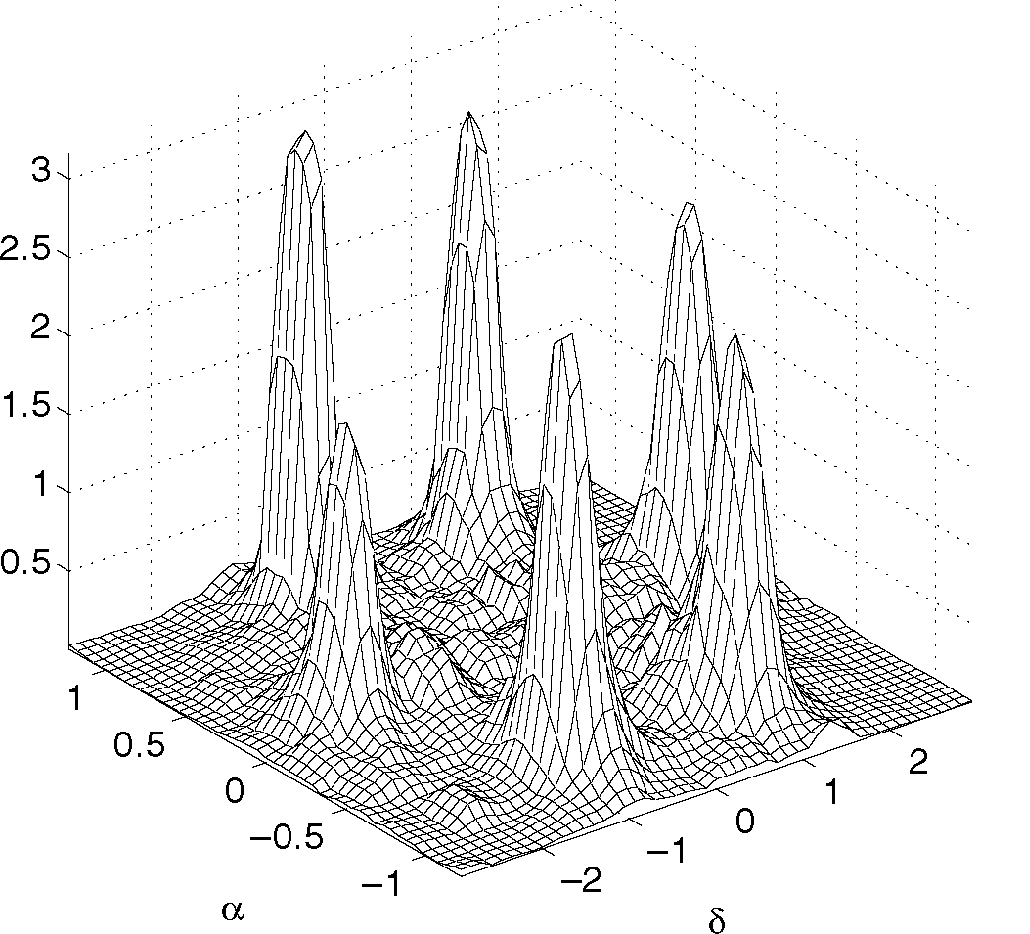
\includegraphics[width = 0.6\linewidth]{./figures/autres/DUET_histogram.png}
\caption{Histogramme 2D pour un signal sonore composé de 6 sources sonores, générant 6 pics \cite{yilmaz2004blind}.}
\label{fig:DUET_hist}
\end{figure}

Une implémentation de cet algorithme, pour une utilisation en temps réel, est proposée \cite{rickard2001real}.
Afin de s'extraire des conditions strictes imposées par la méthode et de s'approcher d'applications plus réelles, \cite{rickard2007duet} propose de considérer l'ajout d'un terme de bruit à l'équation \ref{eq:algo-DUET} et de déterminer l'\textit{atténuation symétrique} $\alpha_j$ et le \textit{déphasage symétrique} $\delta_j$ de chaque source :

\begin{equation}
\alpha_j = \frac{\iint_{(\omega,\tau)} \vert X_1(\omega,\tau) X_2(\omega,\tau)\vert ^p \omega^q \alpha(\omega,\tau) d\omega d\tau}{\iint_{(\omega,\tau)}\vert X_1(\omega,\tau) X_2(\omega,\tau)\vert ^p \omega^q d\omega d\tau},
\end{equation}

avec $\alpha(\omega,\tau) = \bigg\vert \frac{X_2(\omega,\tau)}{X_1(\omega,\tau)} \bigg\vert - \bigg\vert  \frac{X_1(\omega,\tau)}{X_2(\omega,\tau)} \bigg\vert$ et

\begin{equation}
\delta_j = \frac{\iint_{(\omega,\tau)} \vert X_1(\omega,\tau) X_2(\omega,\tau)\vert ^p \omega^q \tilde{\delta}(\omega,\tau) d\omega d\tau}{\iint_{(\omega,\tau)}\vert X_1(\omega,\tau) X_2(\omega,\tau)\vert ^p \omega^q d\omega d\tau},
\end{equation}

Ces deux indicateurs dépendent de deux constantes définies, $p$ et $q$ qui permettent de pondérer le poids de chaque point temps-fréquence :

\begin{itemize}
\item $p$ = 0, $q$ = 0 revient à l'algorithme DUET original,
\item $p$ = 1, $q$ = 0 est motivé afin de donner plus de poids à $\alpha_j$ \cite{yilmaz2004blind},
\item $p$ = 1, $q$ = 2 est motivé afin de donner plus de poids à $\delta_j$ \cite{yilmaz2004blind},
\item $p$ = 2, $q$ = 2 est adapté aux signaux ayant un faible rapport signal à bruit ou bien pour des mixtures de paroles \cite{melia2007underdetermined}.\\
\end{itemize}

Différentes applications basées sur cet algorithme existent notamment pour des signaux de paroles \cite{yilmaz2004blind, jourjine2000blind}.
Plusieurs développement ont été proposés afin d'étendre l'utilisation de cette méthode : dans  \cite{melia2007underdetermined} plusieurs versions sont décrites et comparées dont la \textit{echoic DESPRIT} qui propose avec $M$ microphones de retrouver $N$ signaux (en supposant que le nombre de chemins empruntés par les signaux est inférieur à $\sfrac{M}{2}$) ou bien, dans la variante \textit{echoic ESPRIT}, que le nombre de sources actives simultanément n'excède pas $\sfrac{M}{2}$. \\

%Basée sur une hypothèse d'anéchoïcité, malgré des extensions pour s'affranchir de celle-ci, elle reste peu évidente et adaptée pour un environnement sonore urbain où le champs diffus est prépondérant.

\section{Analyse en Composantes Indépendantes}
L'Analyse en Composantes Indépendantes (ACI) \cite{comon_independent_1994, jutten1991blind} est une méthode appartenant aux méthodes dites de \textit{séparation de sources aveugle}, c'est-à-dire qui sépare un ensemble de sources sonores d'une mixture sans (ou avec peu) informations sur celles-ci. L'illustration la plus couramment citée, pour cette méthode, est l'effet \og cocktail party \fg{}. Cet effet résume le processus qui permet à un être humain de séparer la voix de l'interlocuteur, avec qui il discute, du flux sonore environnant composé d'autre discussions, de musique\dots{} Cette capacité est notamment permise par l'indépendance entre le signal \textit{voix} et les autres sources sonores aux alentour ainsi que par l'écoute binaural du sujet. L'ACI se base sur ces hypothèses pour construire son modèle et s'exprime alors sous la forme d'un produit matriciel :

\begin{equation}\label{eq:ACI2}
\mathbf{x} = \mathbf{As}
\end{equation}

où $\mathbf{x}$, de dimensions $N \times 1$, exprime l'ensemble des mesures faites par des capteurs, $\mathbf{s}$, de dimensions $N \times 1$, résume les différentes sources présentes et $\mathbf{A}$, de dimensions $N \times N$, une matrice déterministe résumant les aspects de propagation entre les sources et les capteurs.
$\mathbf{A}$ et $\mathbf{s}$ étant inconnus, plusieurs hypothèses sont considérées afin de résoudre le problème : i) $\mathbf{s}$ est composé de sources sonores indépendantes, ii) les sources sonores ne suivent pas de distribution gaussienne (ou pas plus de une), iii), $\mathbf{A}$ est une matrice carré inversible. Le problème s'exprime alors sous la forme :

\begin{equation}
\mathbf{s} = \mathbf{A}^{-1}\mathbf{x}.
\end{equation}

L'ACI peut être vu comme une extension de l'Analyse en Composante Principale (ACP) où il y est supposé, non pas l'indépendance des composantes, mais leur décorrélation et où sont déterminer les grandeurs qui ont le plus de variances. L'ACI est donc une méthode plus contrainte (des variables indépendantes seront toujours décorrélées alors que l'inverse n'est pas vraie).
De nombreux développements ont été proposés afin d'obtenir une indépendance maximale entre les sources :

\begin{itemize}
\item la minimisation de l'information mutuelle \cite{hyvarinen97independentcomponent} qui consiste à maximiser un calcul de distance (au travers d'une divergence de Kullback-Leilbler) entre l'entropie de l'ensemble des composantes et d'une composante $i$,
\item la décorrélation non-linéaire qui consiste à minimiser la corrélation deux composantes $y_i$ et $y_j$ chacune exprimée par une fonction $f(y)$ et $g(y)$ dont au moins une est non-linaire (polynôme de degré 2 ou plus, fonction tangente hyperbolique). Pour passer de la non-corrélation à l'indépendance, \cite{jutten1991blind} ajoute une condition où la fonction non-linéaire (ou une des deux)  est impaire avec une moyenne nulle.
\item la minimisation de la \og gaussianité \fg{} des composantes, basée sur le \textit{Théorème Centrale Limite} qui démontre que la somme de variables aléatoires indépendantes forme un ensemble gaussien. La recherche de l'indépendance des sources revient alors à minimiser la \og gaussianité \fg{} entre les composantes. Cette approche est la base de la mesure de la négentropie (ou entropie relative) \cite{lee2000unifying} ou de l'algorithme FastICA \cite{hyvarinen1999fast} qui est l'algorithme le plus couramment utilisé pour résoudre l'ACI.
\end{itemize}

Une large revue exhaustive des méthodes employées est effectuée dans \cite{hyvarinen2004independent}.
Pour être résolue, l'ICA est, le plus souvent, sur-déterminée, ce qui signifie qu'il y a au moins autant de signaux captés que de sources sonores. Pour obtenir une matrice $\mathbf{A}$ carrée, une ACP peut être utilisée afin de supprimer les informations redondantes.  Le cas de la sous-détermination a toutefois été étudié, par exemple dans \cite{bofill2000blind} en considérant les signaux comme parcimonieux.
L'ACI a trouvé de nombreuses applications, en tant que méthode de séparation de sources aveugle, dans le domaine médical, pour extraire les différentes composantes d'un signal d'électroencéphalogramme \cite{delorme2007enhanced,makeig1996independent} ou d'une IMR \cite{lee1999independent}, pour traiter des signaux contenant de la parole \cite{sarela2005denoising, hsieh2009independent} ou pour des contenus musicaux \cite{uhle2003extraction, abdallah2003independent}. Des utilisations de l'ACI pour des sons environnementaux existent aussi \cite{lombard2011tdoa, eronen2006audio}. Cette méthode peut également être utilisée pour des antennes acoustiques et pour la formation de voie (\textit{beamforming})\cite{cardoso_blind_1998,saruwatari2003blind}.

La détermination des matrices $\mathbf{A}$ et $\mathbf{s}$ n'est toutefois pas sans générer des ambiguïtés bien identifiées dans la littérature. La première est l'\textit{ambiguïté de permutation} qui traduit la variabilité dans l'ordre de détermination des composantes indépendantes : une composante estimée $s_1$ peut être déterminé à un rang différent sans pour autant changer la reconstruction du signal global.  Ce problème est toutefois sans conséquence la plupart du temps. Une seconde limite est l'\textit{ambiguité d'échelle} qui traduit la possibilité d'avoir un facteur d'échelle présent dans la matrice $\mathbf{A}$ et $\mathbf{s}$ tel que :

\begin{equation}
\begin{bmatrix}
x_{1}\\
\vdots\\
x_{N}
\end{bmatrix} =
\begin{bmatrix}
\alpha_1 a_{11} & \dots & \alpha_1 a_{1N}\\
\vdots & \ddots & \vdots\\
\alpha_N a_{N1} & \dots & \alpha_N a_{NN}
\end{bmatrix}
\times
\begin{bmatrix}
\sfrac{s_{1}}{\alpha_1}\\
\vdots\\
\sfrac{s_{N}}{\alpha_N}
\end{bmatrix}
\end{equation}

La détermination de l'amplitude exacte des signaux est donc soumise à l'incertitude \cite{naik2011overview}.

\section{Factorisation en Matrices Non-négatives}

La Factorisation en Matrices Non-négatives (abrégé NMF pour \textit{Non-negative Matrix Factorization} en anglais) \cite{lee_learning_1999}, appliquée à l'analyse d'un signal audionumérique, est une méthode qui est basée sur une représentation linéaire de données :

\begin{equation}
\mathbf{V} \approx \mathbf{\tilde{V}} = \mathbf{WH}
\end{equation}

où $\mathbf{V}$ est le spectrogramme en amplitude ou en puissance d'un signal audio de dimensions $F \times N$, $\mathbf{W}$ est appelé \textit{dictionnaire} ou \textit{base}. De dimensions $F \times K$, il contient un ensemble de spectres sonores. $\mathbf{H}$ est la matrice d'activation qui traduit les variations dans le temps de chaque spectre de $\mathbf{W}$.  $K$ définit le rang des matrices et est le plus souvent choisi tel que $F\times K + K \times N \ll F \times N$ afin d'être une méthode qui permet la réduction de données.
Là où l'ACI impose une contrainte d'indépendance, la NMF impose celle de la \og non-négativité \fg{} ($\mathbf{V}$, $\mathbf{W}$ et $\mathbf{H} \in \mathbb{R}_+$). Cette contrainte n'autorise alors que des combinaisons additives entre les composantes et leur assure ainsi d'appartenir au même domaine et donc de leur interprétabilité.
L'approximation entre $\mathbf{V}$ et $\mathbf{WH}$ est résolue en minimisant leur $\beta$-divergence :

\begin{equation}\label{eq:d_v_wh}
\text{min}~D_{\beta}\left(\textbf{V} \vert\vert \textbf{WH}\right) \quad \text{avec} \quad \mathbf{W} \geq 0, \mathbf{H} \geq 0
\end{equation}

Plusieurs approches existent afin de résoudre le problème \ref{eq:d_v_wh}, basées sur des approches itératives : mise à jours multiplicatives \cite{lee_algorithms_2000}, méthode des moindres aux carrés alternés \cite{cichocki_regularized_2007}, gradient projeté \cite{lin_projected_2007} \dots{} La NMF permet aussi d'ajouter des contraintes sur chaque matrice \cite{virtanen_monaural_2007} afin de forcer un type de comportement particulier des matrices suivant le problème posé.

Cette méthode a reçue une grande popularité en trouvant de nombreuses applications pour la musique (transcription de partitions de musique \cite{smaragdis_non-negative_2003,bertin2009tempering}, classification de genre musicaux \cite{panagakis2008music} et d'instruments \cite{benetos2006musical}) et pour la parole (débruitage \cite{wilson2008speech,sprechmann2014supervised}, séparation de sources \cite{smaragdis2007convolutive,
hurmalainen2012detection})\dots{}
Cette méthode a également déjà été confrontée à des sons environnementaux pour différentes tâches comme dans \cite{kumar2016audio} où la NMF est utilisée afin de localiser l'origine de différents extraits sonores. Dans \cite{sobieraj2017masked}, la NMF sert à la détection d'oiseaux dans différents environnements sonores. Dans \cite{heittola_sound_2011}, la NMF est utilisée en vue de détecter plusieurs évènements sonores émis simultanément en représentant les évènements à travers des Chaines de Markov Cachés (HMM) et des Mel Frequency Cepstral Coeffcient (MFCC).  Enfin dans \cite{satoshi_innami_nmf-based_2012}, la NMF est utilisée en tant que méthode de séparation de sources pour extraire différents signaux (voix, aboiements de chien, croassements de grenouille).
Par son fonctionnement, la NMF présente l'avantage, en plus de prendre naturellement en compte le recouvrement temporel entre les sources sonores, d'être adaptée à des réseaux de capteurs monophoniques.

Emmanuel a fait un travail consequent dans le domaine, as-tu bien cite son travail ?

\section{Autre approche : la détection d'anomalies}

Cette approche n'est pas une méthode de séparation de source puisque l'objectif est d'identifier les sources sonores qui composent une mixture sonore pour ensuite ne considérer que celles d'intérêts.

La reconnaissance et la détection de sources sonores environnementales à l'aide de descripteurs \cite{dufaux2000automatic,defreville_automatic_2006} reçoit une attention croissante. Ces travaux suivent le plus souvent un protocole établi : i) apprentissage d'un détecteur sur une base de données, ii) application de ce détecteur sur une base de test en vue d'estimer les performances de l'outil. Dans \cite{mesaros2010acoustic}, 61 évènements sonores sont détectés parmi des enregistrements audio annotés à l'aide de l'algorithme de Viterbi et des HMM. \cite{ntalampiras2011probabilistic} détecte des évènements anormaux tel que des cris, des tirs d'armes à feu à partir de mixtures sonores synthétisées où le niveau sonore de ces évènements est échelonné entre -5 dB et 15 dB. Les descripteurs utilisés sont les MFCC, MPEG-7 et les \textit{Perceptual Wavelet Packets} et le classifieur est basé sur un Modèle de Mixtures de Gaussiennes (GMM) et sur des HMM. Ces travaux seront étendus dans \cite{ntalampiras2014universal} pour réaliser un outil de surveillance du trafic routier. Dans le cadre du projet DYNAMAP, un détecteur d'évènements sonores anormaux (DESA) a été réalisé \cite{socoro2017anomalous} pour identifier les évènements sonores qui ne sont pas reliés au trafic, dans le but de ne pas les considérer dans l'estimation du niveau sonore du trafic routier. Leur outil se base, là aussi, sur les MFCC (13 bandes), exprimés sur des trames temporelles de 30 ms, couplés à des GMM. Le corpus de test est divisé en deux classes : \textit{urbain} et \textit{banlieue}. Les performances du détecteur, évalué au travers du F-score, est pour chaque classe du corpus de 61,5 $\%$ et de 72,3 $\%$.

\section{Comparaison des approches}

Le Tableau \ref{tab:comparaison_method} compare les différents caractéristiques requises par l'outil de séparation de sources afin de satisfaire le cahier des charges proposé dans la partie \ref{part:cachier_charges}. Pour rappel, celui-ci doit être adapté aux sons environnementaux, au phénomène de recouvrement temporel et aux réseaux de capteurs monophoniques.

\begin{table}[ht]
\centering
\caption{Comparaison des 4 méthodes de séparation de sources pour estimer le niveau sonore du trafic routier à partir d'un enregistrement monophonique.}
\label{tab:comparaison_method}
\begin{tabular}{lcccl}
\toprule
adapté & \begin{tabular}[c]{@{}c@{}} sons \\ environnementaux\end{tabular} & \begin{tabular}[c]{@{}c@{}}recouvrement \\  temporel\end{tabular} & \begin{tabular}[c]{@{}c@{}} réseau de capteurs\\  monophoniques\end{tabular} &  \\
\midrule
CASA & - & + & - &  \\
\cellcolor[HTML]{C0C0C0}Algorithme DUET & \cellcolor[HTML]{C0C0C0}- & \cellcolor[HTML]{C0C0C0}+ & \cellcolor[HTML]{C0C0C0}- &  \\
ACI & + & ++ & - &  \\
\cellcolor[HTML]{C0C0C0}NMF & \cellcolor[HTML]{C0C0C0}++ & \cellcolor[HTML]{C0C0C0}++ & \cellcolor[HTML]{C0C0C0}++ &  \\
DESA  & ++ & + & ++ & \\
\bottomrule
\end{tabular}
\end{table}

En conclusion, la méthode CASA et l'algorithme DUET sont des méthodes qui sont peu adaptées au cas d'étude présent, car elles sont développées notamment pour des sons harmoniques et qui nécessitent au minimum, deux microphones pour chaque point de mesure. Pour la même raison, l'ACI n'est pas une méthode adaptée à la mise en place de réseaux de capteurs monophoniques. De plus l'\textit{ambiguité d'échelle} est un frein pour estimer correctement le niveau sonore du trafic. L'outil DESA répond à une grande partie des besoins, mais, comparé à la NMF, ne gère pas aussi bien le problème du recouvrement temporel, où à un instant $t$, un évènement est classé soit \textit{trafic} soit \textit{anormal}. Or dans certain cas, le recouvrement peut être très important et s'étendre dans la durée. Cette approche étant susceptible de mettre de coté trop d'échantillons, c'est donc, la NMF qui, au vue de son fonctionnement (reconstruire le spectrogramme d'un signal à l'aide d'un dictionnaire), nous paraît être la méthode la plus adaptée au cadre de cet étude.

%\section{Formation de voies ou \textit{beamforming}}
%
%La formation de voies est une méthode de traitement du signal qui permet, à partir d'un ensemble de microphones, de déterminer les contributions respectives de plusieurs sources sonores. Cette méthode est couramment utilisée pour des antennes acoustiques. Le principe de la méthode réside dans la création d'un vecteur de pointage dans une direction donnée où on cherche à localiser une source sonore. Ce vecteur de pointage permet alors de pondérer le signal de chaque microphone pour ensuite les sommer. Plusieurs méthodes peuvent être employé pour construire ce vecteur de pointage :
%
%\begin{itemize}
%\item par déphasage soit temporel entre les signaux, soit à une fréquence donnée,
%\item par optimisation soit en minimisant une fonction cout entre les mesures de chaque microphone et la source sonore (processeur de Bartlet), soit en minimisant les variances entre les énergies des différentes sources (méthode de Capon)
%\item par méthodes de \og hautes résolutions \fg{} où une décomposition en sous-espace des matrices spectrales pour chaque pair de microphone est réalisée et qui par orthogonalité permet de séparer les sources du bruits ou bien par la décomposition aux valeurs propres (MUSIC) qui permet également de déterminer la présence d'une source en un point $i$.
%\end{itemize}
%
%Cette méthode est couramment utiliser pour réaliser de la localisation de sources sonores où les effets Doppler sont à prendre en compte dans la chaine de traitement \cite{ward1998space,chen2002source,mennitt2010multiple}.

%%%%%%%%%%%%%%%%%%%%%%%%%%%%%%%%%%%%%%%%%%%%%%%%%%%%%%%%%%
%\section{Séparation de sources à partir d'un signal monophonique}
%
%Ces méthodes visent à répondre à la problématique suivante : comment peut-on extraire les différentes sources sonores qui compose notre signal audio monophonique ? Plusieurs approches existent : soit partir du signal global et essayer de déterminer les sources qui le compose (approche dite \textit{top-down}), soit considérer des sources, connues \textit{a priori} ou apprises qui vont recomposer le signal mesuré (approche \textit{bottom-up}).
%Les techniques de séparation de sources peuvent se classer en trois catégories : les approches techniques, l'Analyse Computationnelle de Scènes Auditives et les méthodes par dictionnaires
%
%\subsection{L'analyse Computationnelle de Scènes Auditives }

%L'analyse de scènes audio statistique (abrégé CASA pour \textit{Computational Auditory Scene Analysis} en anglais) est une des premières techniques numérique cherchant à séparer les différentes sources composant un signal. Elle fut proposé par Brown \cite{BrownCASA} et se base sur la simulation de la réponse auditive d'un humain.\\
%
%
%
%La CASA construit son modèle sur l'architecture de l'oreille. Elle se décompose en 4 parties :
%
%\begin{itemize}
%\item un filtrage du signal capté,
%\item une analyse temps-fréquence,
%\item une cartographie du signal,
%\item un groupement d'algorithmes.\\
%\end{itemize}
%
%Maintenant que le son est capté, la seconde étape revient à donner un sens au son. Pour cela, le cerveau s'aide des sons capté par les deux oreilles, par les informations temps-fréquences qu'il saura etraire du signal et de son apprentissage.\\

%Pour localiser une source, l'humain se sert de ces deux oreilles. Il se forme alors un déphasage temporelle entre les deux signaux captés (\textit{interaural time difference}, ITD) qui fourni un premier indice sur la localisation de la source. Également, l'oreille la plus proche de la source sera susceptible d'avoir un niveau sonore plus important (\textit{interaural intensity difference}, IID). Cette différence de niveau sonore entre les deux oreilles aide alors à mieux définir la localisation de la source. Dans les basses fréquences (inférieur à 500 Hz), l'IID ne fournit pas d'informations suffisantes à l'inverse de l'ITD. Alors qu'en haute fréquence, c'est l'inverse : l'ITD ne peut pas fournir d'information utile en raison des incertitudes liées à la phase là où l'IID peut être utile.\\



%\subsubsection{Organisation de l'audition et de la perception}
%\begin{figure}[hbtp]
% \centering
% 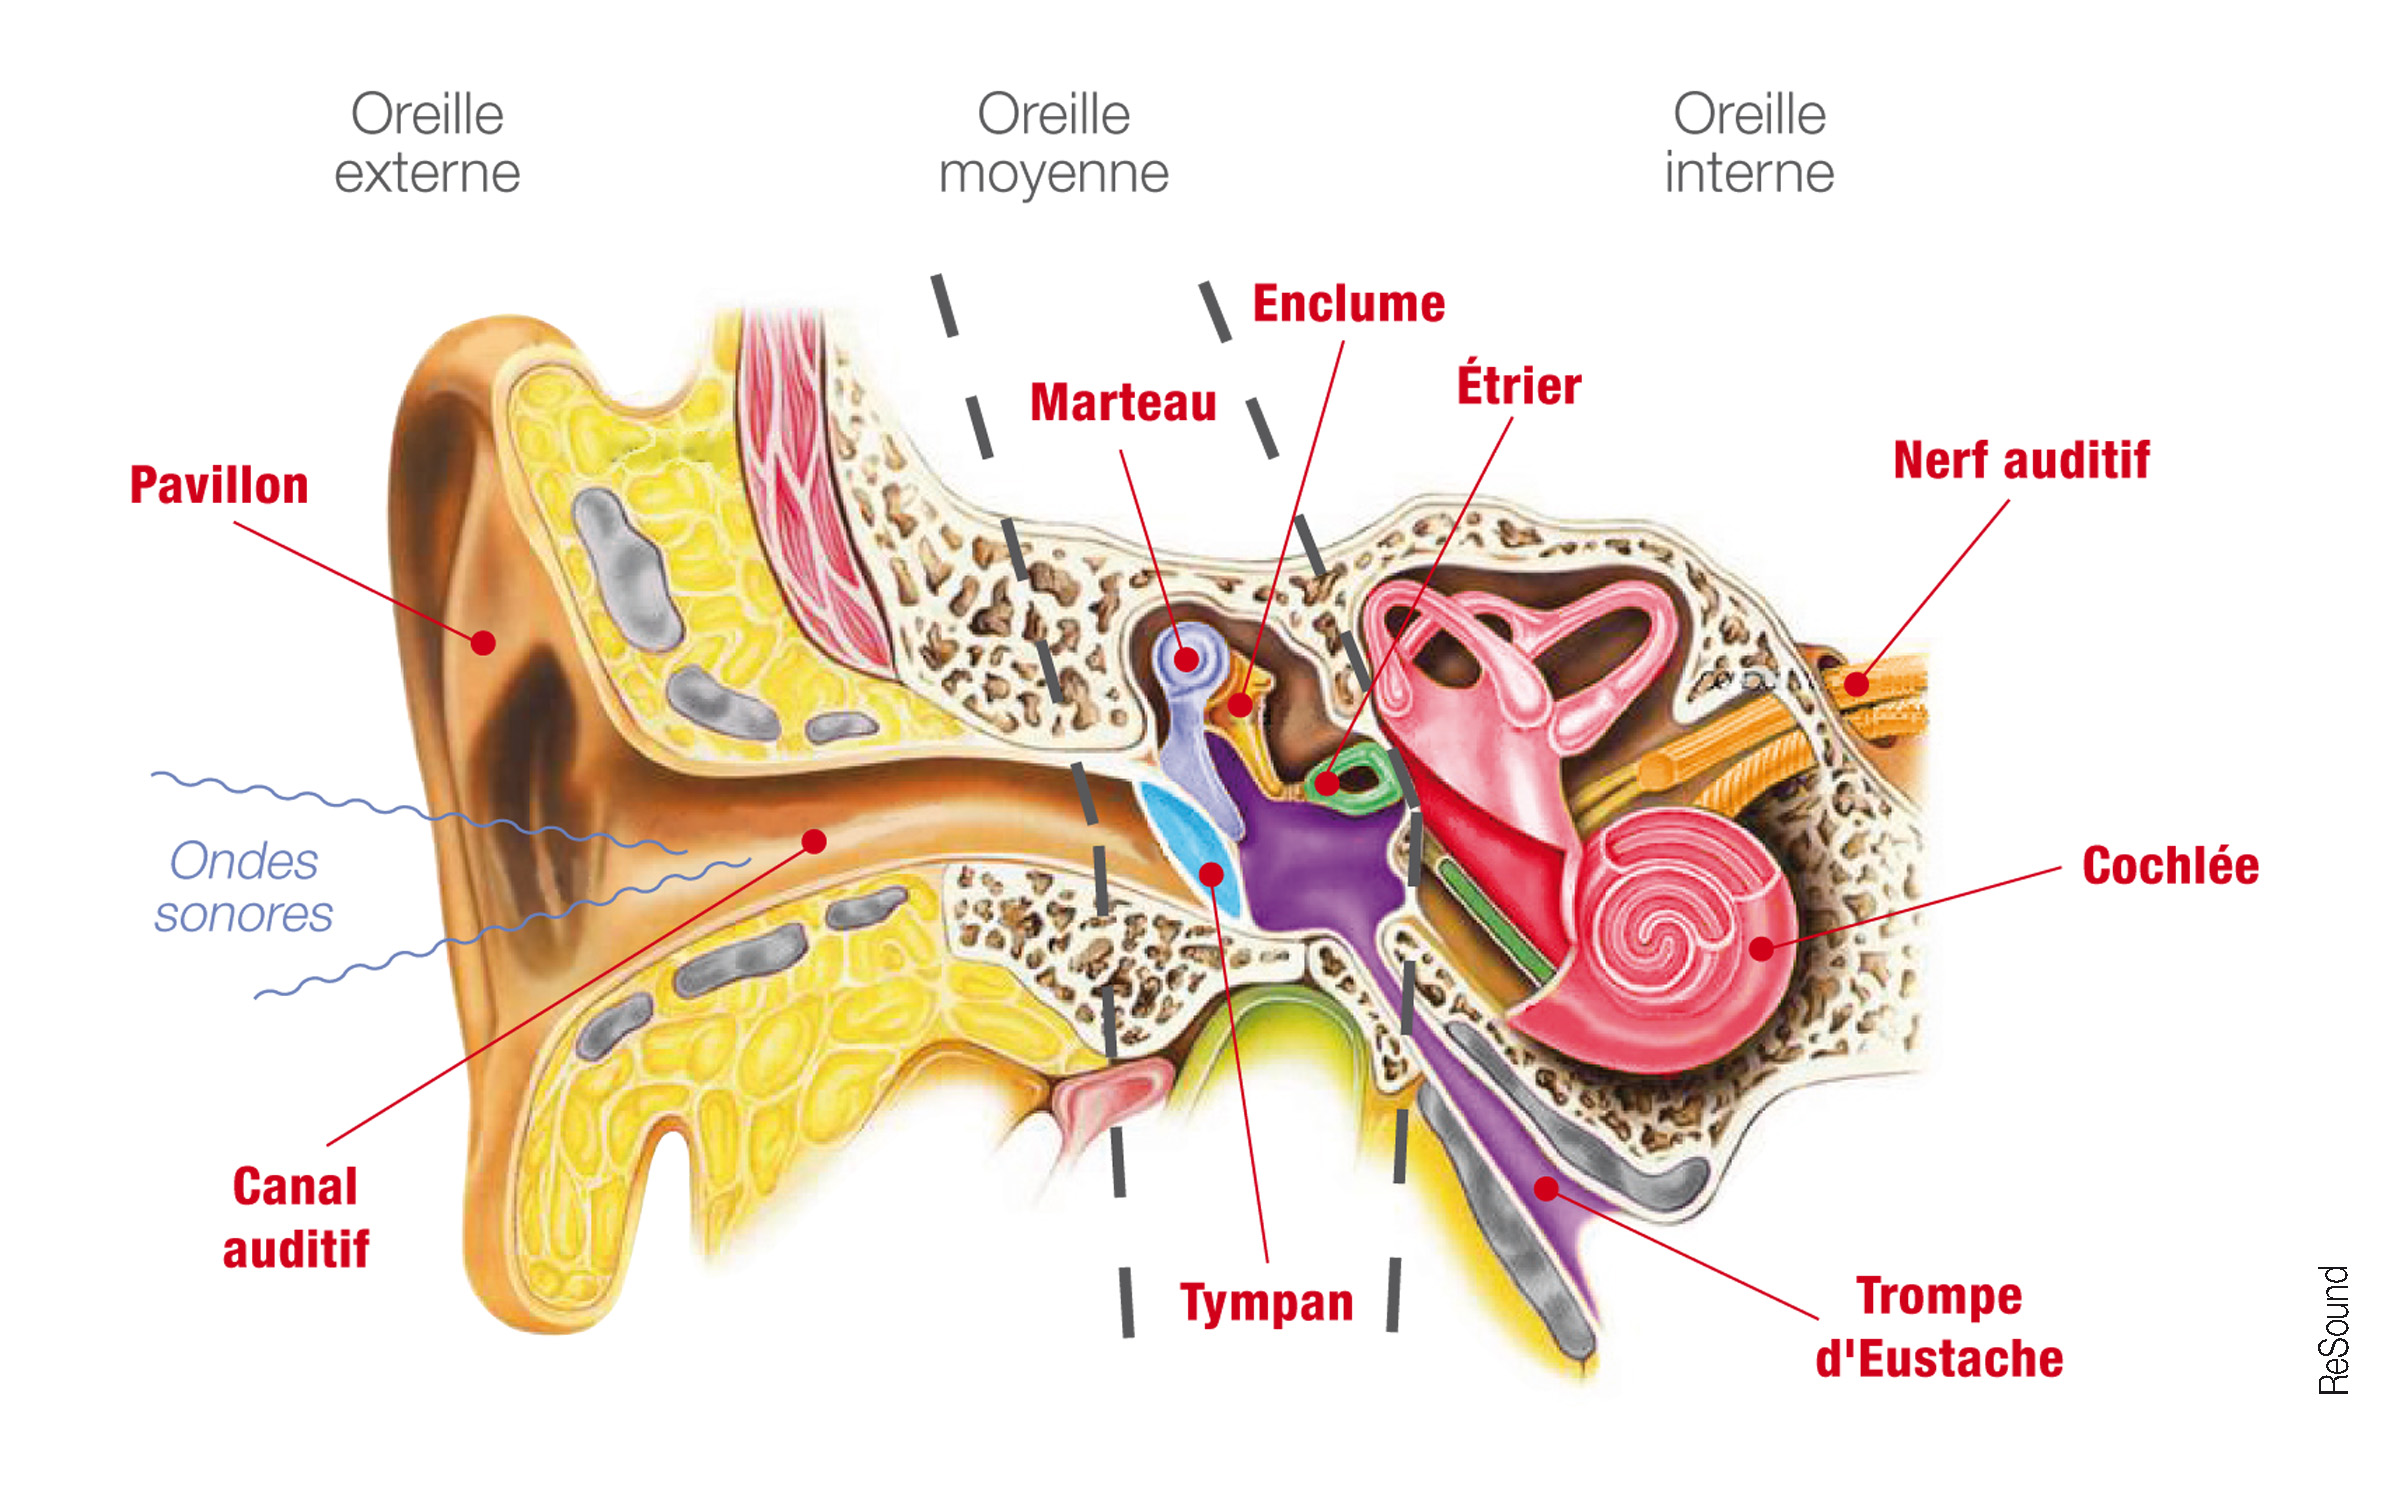
\includegraphics[width=0.8\textwidth]{../../../../Pictures/OREILLE.jpg}
% \caption[width=0.5\textwidth]{Schéma de l'oreille interne (http://www.mon-audition.info/wp-content/uploads/2015/01/OREILLE.jpg)}
% \label{fig:schemaOreille}
%\end{figure}

%L'oreille humaine est composé de trois parties ayant chacune leur fonction : l'oreille externe  qui permet la localisation des sources, l'oreille moyenne qui joue le rôle d'amplification du son et l'oreille interne qui traduit la pression acoustique du signal en un signal électrique interpréter par le cerveau. Si le tympan et les osselets jouent le rôle d'adaptateur d'impédance entre l'extérieur et l'oreille interne, c'est la cochlée qui permet d'obtenir un signal électrique qui sera transmise au cerveau via le nerf auditif. \\

%\begin{figure}[hbtp]
% \centering
% 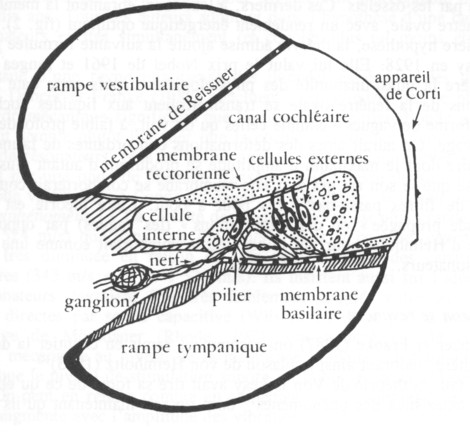
\includegraphics[width=0.4\textwidth]{../../../../Pictures/cochlea.jpg}
% \caption{Schéma en coupe d'une cochlée (http://auriol.free.fr/psychosonique/ClefDesSons/ecoute.htm)}
% \label{fig:schemaCochlé}
%\end{figure}

%La cochlée consiste en une spirale creuse traversé par le canal cochléaire composé notamment de la membrane basilaire sur laquelle repose l'organe de Corti. Lorsqu'une onde acoustique arrive au tympan, elle est converti en énergie mécanique dont l'énergie est ensuite transmise à la cochlée grâce au osselets. Cette énergie met en mouvement la membrane basilaire à des positions localisées qui dépendent de la fréquence du signal. Par ce déplacement, les cellules cilié se trouvant dans l'organe de Corti vont alors bouger convertissant le signal mécanique en en signal électrique qui se propage ensuite jusqu'au cerveau à travers le nerf auditif (http://www.cochlea.eu/cochlee). C'est ensuite dans le cerveau que le son est interprété et que l'auditeur peut y mettre un sens. Pour cela, les évolution des caractéristiques acoustiques (niveau sonore, continuité temporelle et fréquentielle) du son aide à la compréhension et la distinction des sources présentes. \\
%
%La CASA reprend donc ces éléments et cherche à traduire ces organes en étapes numériques, la première étant la modélisation de l'ensemble oreille externe/moyenne/interne.\\

%\subsubsection{Analyse fréquentielle}
%
%L'oreille externe et moyenne sont résumées en un simple filtre passe-haut. Ensuite, l'oreille interne est synthétisée par un filtrage cochléaire (cochléogramme). Ce filtre traduit la sélectivité fréquentielle de la membrane basilaire en la modélisant par une banque de filtres passe-bandes dans laquelle chaque filtre simule la réponse en fréquences d'un point particulier de la partition cochléaire. Les cellules ciliées étant les éléments dans la membrane qui transmettent les perturbations vers le nerf auditif, leur réaction est modélisée par un filtre de gammatone basé sur un filtre impulsionnel.\\
%
%\begin{equation}
%gt(t) = t^{n-1} e^{-2\pi bt } \cos(2\pi f_0 t+\phi)
%\end{equation}
%
%avec $t$, le temps en seconde, $n$, l'ordre du filtre, $f_0$, la fréquence centrale du filtre en Hz, $b$ la largeur de la bande passante en Hz et $\phi$ la phase (rad). En sortie de la cochlée, on préfère utilisé comme représentation temps-fréquence, un cochléogramme au spectrogramme qui permet de mieux mettre en évidence les basses fréquences grâce à une échelle logarithmique.\\
%
%\subsubsection{Paramètre d'extraction}
%
%Cette seconde étape vise à extraire plusieurs paramètres qui seront utile à l'étape de groupement (partie \ref{sec:groupement}) :
%
%\paragraph{Pitch et périodicité}
%L'objectif consiste à déterminer les fréquences fondamentales et les phénomènes récurrent à partir de l'auto-corrélations $a(t,f,\tau)$ pour chaque oreille (corrélogramme) et de l'inter-corrélation $c(t,f,\tau)$ entre les signaux des deux oreilles $h_L$ et $h_R$(corrélogramme-croisé).
%
%\begin{equation}\label{eq:CASA_FAC}
%a(t,f,\tau) = \sum h(t-n,f)h(t-n-\tau,f)w(n),
%\end{equation}
%
%\begin{equation}\label{eq:CASA_FAC}
%c(t,f,\tau) = \sum h_L(t-n,f)h_R(t-n-\tau,f)w(n).
%\end{equation}
%
%La somme pour chaque fréquence permet alors de déterminer les fréquences fondamentales présentes
%
%\begin{equation}
%A(t,\tau) = \sum_f a(t,f,\tau),
%\end{equation}
%\begin{equation}
%C(t,\tau) = \sum_f c(t,f,\tau).
%\end{equation}
%
%Si plusieurs sources sonores sont simultanées et présente des différentes fréquences fondamentales, il existe un moyen pour les déterminer \cite{DeCheveigne20006}.
%\paragraph{Corrélation croisée des voix}
%Comme les réponses des filtres gammatone se recouvrent, plusieurs bandes peuvent réagir à une même harmonique. La corrélation autour des fréquences voisines permet alors de mieux connaitre le phénomène. celle-ci se définit comme l'inter-correlation au fréquences voisines des auto-corrélation normalisées.
%\begin{equation}
%k(t,f) = \frac{1}{M}\sum_{\tau=0}^{M-1}\hat{a}(t,f,\tau) \hat{a}(t,f+1,\tau)
%\end{equation}
%\paragraph{Variation de l'intensité}
%L'apparition ou la disparition de sources sonores pouvant d'accompagner d'une variation du niveau sonore. Des valeurs seuils sont déterminées pour détecter ces variations à partir de la dérivée de l'enveloppe du signal.
%
%\paragraph{Modulation d'amplitude}
%L'extraction des modulation d'amplitude des enveloppes permet de revenir à l'enveloppe du signal même. Une des méthodes couramment employé est l'utilisation des transformée de Hilbert ou bien l'amplitude absolue des signaux en sortie des filtres complexes de gammatone.
%
%\paragraph{Modulation de fréquence}
%Ce paramètre permet de rendre compte des régimes transitoires.  Deux techniques existent, la première méthode consiste revient à extraire les contours spatiales du cochléogramme, la seconde implique de calculer la réponse fréquentielle instantanée des signaux en sortie des filtres passe-bandes.
%
%\subsubsection{Représentation à niveau moyen}
%Cette étape consiste à établir une représentation des paramètres précédents le plus souvent par segmentation.
%\subsubsection{Groupement des sources}\label{sec:groupement}
%
%\subsubsection{Re-synthétisation}
%
%
%
%La cartographie du signal permet ensuite de retrouver le signal perçu par l'auditeur. Elle se base sur des fonctions de corrélations (corrélogramme) visant à synthétiser les phénomènes de masquage et à faire ressortir les pics principaux des signaux
%Enfin un second corrélogramme entre les signaux issus des deux microphones (simulant les deux oreilles) permettent la localisation des sources grâce à leur déphasage.

%\subsection{Les méthodes par dictionnaires}
%
%\subsubsection{Analyse en Composantes Indépendantes}\label{part:ACI}
%
%L'Analyse en Composantes Indépendantes (ACI) \cite{Herault} \cite{Comon} est une méthode appartenant aux méthode dite \textit{séparation de sources en aveugles}, c'est-à-dire qui sépare un ensemble de sources sonore d'une mixture sans (ou avec peu) informations sur celles-ci. Le plus souvent, cela équivaut à résoudre un problème sous déterminé. Le principe de la méthode consiste, à partir d'un réseau de capteurs, à trouver les sources présentes dans un signal audio en supposant leur indépendances les unes des autres. \\
%
%
%
%L'ACI consiste alors à décrire les signaux de chaque capteur $x_n$ comme une combinaison linéaires des sources $s_n$ présentes, supposées indépendantes et pondérées par des effets propagatifs $a_{nn}$. Dans le cas du \og cocktail party \fg{}, on considère deux signaux (la voix et le bruit) où les capteurs sont les deux oreilles de l'auditeur.
%
%\begin{subequations}\label{eq:ACI1}
%\begin{align}
%x_1 &= a_{11} s_1 + a_{12} s_2 + \dots + a_{1N} s_N\\
%x_2 &= a_{12} s_1 + a_{22} s_2 + \dots + a_{sN} s_N\\
%x_n &= a_{n1} s_1 + a_{n2} s_2 + \dots + a_{nN} s_N
%\end{align}
%\end{subequations}
%
%Le système \ref{eq:ACI1} est alors généralisé à un ensemble $N$ de sources par l'équation~(\ref{eq:ACI2}).
%
%\begin{equation}\label{eq:ACI2}
%\mathbf{x} = \mathbf{As}
%\end{equation}
%
%où $\mathbf{x}$ est de dimension $P \times 1$ comprenant l'ensemble des mesures réalisées par les capteurs, $\mathbf{s}$, de dimension $N \times 1$, résume les différentes sources présentes et $\mathbf{A}$, de dimension $P \times N$, une matrice déterministe résumant les aspects de propagation entre les sources et les capteurs. Cet aspect peut se révéler très intéressant lorsque les milieux dans lesquels évoluent les signaux sont complexes. Toutefois, l'estimation de la matrice $\mathbf{s}$ ne peut se faire que si le nombre de capteurs est égale ou supérieur aux nombres de sources présentes ($P \geq N$).\\
%
%Le problème à résoudre devient alors
%
%\begin{equation}
%\text{min } I(\mathbf{A}^{-1}\mathbf{x})
%\end{equation}
%
%où $I(\mathbf{y})$ est une mesure de dépendance des coordonnées de la matrice $y$. Sa minimisation assure la meilleure indépendance possible des solutions du problème.
%Il y a indépendance entre les sources lorsque
%\begin{equation}
%p(\mathbf{x}) = \prod_{i = 1}^N p(x_i).
%\end{equation}
%où $p(\mathbf{x})$ est une fonction de densité de probabilité de $\mathbf{x}$. La mesure d'indépendance est ensuite déterminée par le calcul de la divergence de Kullback-Leibler que Comon \cite{Comon} a choisi en raison de ces propriétés.
%
%\begin{equation}\label{eq:divKLICA}
%D(\mathbf{y}) = \int p(\mathbf{y})\log\frac{p(\mathbf{y})}{\prod_{i = 1}^N p(y_i)} d\mathbf{y}.
%\end{equation}
%
%La minimisation de (\ref{eq:divKLICA}) rend alors les composantes moins dépendantes les unes des autres. Toutefois, il n'existe pas d'algorithme générique qui permettrait de résoudre le problème facilement \cite{CichockiICA}, des connaissances \textit{a priori} sur les sources ou sur l'environnement sont nécessaires pour exprimer au mieux l'indépendance comme l'évolution temporelle ou spatiale des signaux.  \\
%
%
%Si la technique peut sembler intéressante elle présente l'inconvénient de nécessiter un nombre de capteur égal ou supérieur au nombre de sources présentes. Dans un espace clôt, cette condition est supportable mais, dans le cadre urbain où le nombre de sources est important, cette contrainte rend son utilisation peu envisageable.\\
%
%Les méthodes de séparation couramment utilisées ne sont donc pas des méthodes bien adapté à notre situation et ne peuvent donc pas être utilisé. Néanmoins, une autre technique appartement à la méthode de \textit{BSS} offre des résultats intéressant et prometteur et peut être envisagée pour des ambiances sonores urbaines : la Factorisation en Matrice Non-Négative.

%\subsection{Applications}
%
%L'utilisation de ces techniques dans le domaine de la classification et de la détection se fait couramment et dans des domaines diverses (
%
%Rappeler les applications diverses dans les images, le milieu médicale, textuelles.
%Dans le cadre des signaux audiophoniques :
%séparation des sources sonores afin de réaliser des commandes vocales, de restaurer des signaux audio indépendamment
%paroles, musiques, sons environnementaux...
%
%Dans le cadre de la restauration audio, classifier par genres musicaux, artistes..., traitement actif du son également, reconnaissance ou commande vocale.
%Les sons environnementaux sont constitués des sons qui ne sont ni musicaux ni de la paroles. On trouve dedans les sons produits par l'Homme (bruit mécaniques) ou ceux produit par les animaux (bio-acoustique). Ce choix de distinctions provient de la nature des sons qui est beaucoup plus harmonique dans la parole et la musique que dans l'environnement.\\
%
%Dans le cadre des sons urbains, on trouve des études portant sur la reconnaissance des sons présents en ville (Defréville, Couvreur)%\section{Méthodes de détection et d'identification}
%\label{sec:ident_detec}
%
%Lorsqu'on parle de classification, il s'agit de savoir automatiquement savoir si un extrait audio appartient à une catégorie ou à une autre. Il peut s'agir de classer un morceau de musique selon son style \cite{tzanetakis_musical_2002}, de classer un enregistrement sonore selon son environnement sonore \cite{chu_where_2006}. Lorsqu'on parle de détection, on parle de la détermination du temps de présence des différents évènements sonores dans un scène sonore mais également à déterminer la source sonore correspondante. Cette tâche trouve notamment son intérêt lors des phases d'annotation de scènes sonore où un auditeur estime à la main le temps d'apparition et de fin des différents évènements, tâche qui peut être très fastidieuse et complexe \cite{mesaros_sound_2015} \cite{cakir_polyphonic_2015}. \\
%
%Afin de comparer les performances des algorithmes, plusieurs bases de données on été conçu, lors de challenges, afin d'être utiliser pour les tester. Dans le cas de la parole, la base de données CHiME \cite{christensen_chime_2010} est la plus souvent utilisée \cite{barker_pascal_2013} \cite{araki_2011_2012}. Pour la musique, des bases de données, comme RWC \cite{goto_rwc_2003} et CAL500 \cite{wang_towards_2014}, existent et servent pour des tâches comme la classification par genre musicaux ou à la définition des structures musicales. Certaines base de données sont même destinées à une classe d'instrument particulière (comme les instruments percussifs pour la base de données , ENST-drums \cite{gillet_enst-drums:_2006}). \\
%
%Si ces base de données et challenge on été destiné à la parole et à la musique, c'est à partir de 2013 qu'est crée le challenge \textit{Detection $\&$ Classification of Acoustics Scene Event} (DCASE) \cite{giannoulis_detection_2013} qui s'adresse aux sons environnementaux. La lecture des articles résumant les techniques ainsi que les résultats permet de connaitre les méthodes qui sont plébiscités. \\
%
%
%De nombreux modèles de classificateur ou de détecteur adapté à des sons urbains utilisent les même outils que pour les sons de paroles ou musicaux. Cette partie présente les approches et les différents outils les plus couramment utilisés. Le modèle de classification est réalisée en deux étapes. Les signaux audio sont d'abord décrits par des descripteurs qui vont donner une représentation réduite des classes de sons visées. Un classificateur est ensuite utilisé permettant ainsi de distinguer les différentes classes de sons présentes dans le signal audio. La partie~\ref{part:descripteur} et \ref{part:classificateur} exposent respectivement les différents descripteurs et classificateurs couramment utilisées.
%
%\subsection{Descripteurs}\label{part:descripteur}
%Un large nombre de descripteurs ont déjà été utilisé dans la littérature \cite{} \cite{} \cite{}. Ces descripteurs peuvent décrire un signal à la foi dans le domaine temporel que fréquentiel. Ils permettent de réduire la dimension du signal audio à quelques valeurs simplifiant la classification. Pour être optimal, le choix de ces descripteurs doit permettre une description unique des classes de sons. Dans \cite{}, Peeters résume un grand nombre de paramètres couramment utilisé qu'il regroupe dans le projet CUIDADO. Il classe les paramètres en 5 familles : les paramètres temporels, énergétiques, spectraux, harmoniques et perceptifs.
%
%\begin{itemize}
%\item \textbf{paramètres temporels} : il résume aussi bien les paramètres qui décrive un signal sur des parties entière du signal (par exemple l'attaque, la tenue et l'extinction du isgnal) que de manière instantanée avec la fonction d'auto-corrélation ou le \textit{Zero-Crossing Rate} qui énumère le nombre de fois qu'un signal traverse l'axe des zéro. Un faible ZCR traduit un signal harmonique alors qu'un grand ZCR signifie le son est composé de bruit.
%
%\item \textbf{paramètres énergétiques} : Il résume les indicateurs énergétique aussi bien du signal entier que de partie plus restreinte ou bien encore celles des composantes harmoniques ou du bruits.
%
%\item \textbf{paramètres spectrales} : C'est une classe de descripteurs large. Elle contient des descripteurs simples comme le centre de gravité spectrale ou qui calcule l'évolution temporel du spectre (ou flux spectral) comme des descripteurs plus complexe comme les LPCC (Linear Predictive Cepstral Coefficient) et les MFCC (Mel Frequency Cepstral Coefficient). Les MFCC sont couramment utilisés dans les tâches de classification ou de détection. Ils consistent à exprimer la transformée de Fourier d'un signal par des bandes Mel et à réaliser à transformée en cosinus discret du logarithme du signal obtenu (figure \ref{fig:schema_mfcc}).
%
%%\begin{figure}[h]
%%\centering
%%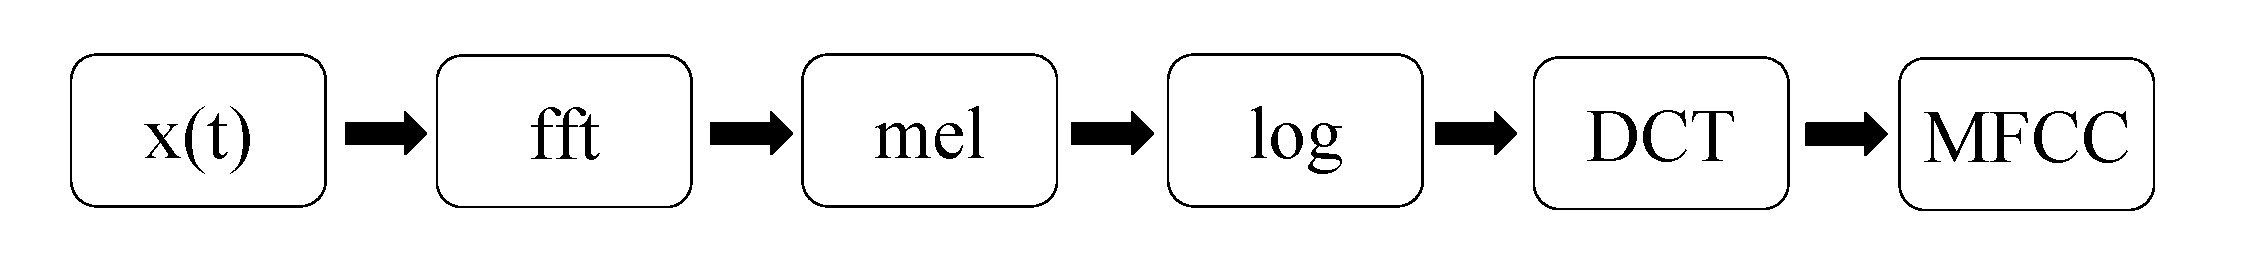
\includegraphics[width = 0.7\textwidth]{./figures/autres/schema_MFCC.pdf}
%%\caption{Schéma de la conception des MFCC}
%%\label{fig:schema_mfcc}
%%\end{figure}
%
%L'échelle Mel est une échelle de hauteur de sons issus de la psycho-acoustique. Son échelle est construite afin qu'un doublement de mel corresponde à un doublement de la fréquence perçu. Par exemple pour un son pur à 1000 Hz (correspondant à 1000 mel), le son perçu deux fois plus aigu sera un son à environ 3428 Hz et non à 2000 Hz. L'échelle des Mel est alors définit par la relation \ref{eq:melScale} permettant ainsi de conserver le rapport 2 entre les deux sons (le signal à 3428 Hz est alors à 2000 mel),
%
%\begin{equation}\label{eq:melScale}
%mel = 1127 \ln\left(1+\frac{f}{700}\right).
%\end{equation}
%
%
%\item \textbf{paramètres harmoniques} : Cette catégorie regroupe des descripteurs comme la détermination de la fréquence fondamental, de  l'inharmonicité ou bien du tristimulus du signal.
%
%\item \textbf{paramètres perceptifs} : Cette dernière classe regroupe les indicateurs psycho-acoustique comme l'acuité ou la sonie du signal.\\
%\end{itemize}
%
%Dans son article, Peeters \cite{Peeters} résume un ensemble de descripteurs couramment utilisés dans le domaine de la reconnaissance de parole \cite{Kim} ou le domaine de la musique \cite{Fu} qui sont ceux qui sont également utilisés pour des ambiances sonores environnementales \cite{Cowling}, \cite{Haddad}, \cite{Defreville}.


%
%En raison de l'utilisation de l'échelle Mel, les MFCC sont le plus souvent utilisés dans le cas de la détection de signaux de paroles \cite{Wu}.

%\subsection{Analyse en Composante Principale}\label{part:ACP}
%
%L'utilisation de plusieurs descripteurs génèrent un ensemble de données décrivant chaque signal spécifiquement.
%
%\begin{equation}
%\mathbf{X} =
%\begin{pmatrix}
%x_{11}& x_{12} & \dots & x_{1p} \\
%x_{21}& x_{22} & \dots & x_{2p} \\
%\vdots & \vdots & \ddots & \vdots \\
%x_{N1}& x_{N2} & \dots & x_{Np}
%\end{pmatrix}
%\end{equation}
%
%où $N$ est le nombre de signaux traités et $p$ le nombre de variable utilisé pour les décrire. Néanmoins, leur représentation graphique en un nuage de point qui permettrait de visualiser la corrélation entre les signaux n'est pas facile au delà de $p = 3$ car la dimension de problème n'est alors plus représentable. De plus, certains paramètres sont parfois redondant et ajoute une dimension aux problème rendant la représentations des corrélations entre elles plus difficile. \\
%
%L'Analyse en Composante Principale (ACP) se propose alors de réduire les dimensions du problème en passant d'un espace à $p$ dimensions à un sous-espace réduit $k$ (le plus généralement $k = 2$ ou $k=3$). Ces nouvelles variables $k$ sont construites à partir de combinaisons linéaire des $p$ variables initiales et celle qui présentent les plus fortes variances. Elles sont appelées \og composante principale \fg{} et forment de nouveaux axes de représentations appelé \og axes principaux \fg{}. Ce choix permet de conserver le plus d'information possible. Pour cela le sous-espace est construit afin que sa distance avec les données de $\textbf{X}$ soit minimale et que la projection du nuage de points est une dispersion (ou inertie) maximale.
%
%L'extraction de paramètres des signaux permet alors d'apporter de nouvelles informations qui vont permettre ainsi de séparer les signaux en fonction des classes de son présentes. Leur choix doit permettre de rendre chaque description des classe unique afin que la classification soit réussie.

%\subsection{Classificateurs}\label{part:classificateur}
%
%L'étape de classification vise à reconnaitre les différentes classes de sons présentes à l'aide des descripteurs offrant ainsi une référence qui permettra la reconnaissance des sources lors de la phase de test. Les méthodes de classification peuvent être considéré par deux approches : discriminative ou générative.\\
%
%La première approche modélisent directement la règle de classification. Les plus populaires sont les \og $k$-plus-proches voisins \fg{} ($k$-NN pour \textit{k-Nearest-Neighbours} en anglais) ou les Vecteurs à Support de Machine (SVM pour \textit{Support Machine Vectors} en anglais). \\
%
%La méthode $\mathbf{k-}$\textbf{NN} consiste à calculer les distances entre un échantillon testé $x$ et les données issus de l'apprentissage. La classe ayant alors les $k$ distances les plus faibles est donc celle de l'échantillon $x$.\\
%
%La méthode \textbf{SVM}, quant à elle, consiste à déterminer un séparateur linéaire entre deux ensembles de telle façon que la distance normal des plus proches échantillons des classes à cette courbe soit maximisée. Cette courbe est appelé \textit{hyperplan} et les échantillons qui maximisent la distance sont les \textit{vecteurs supports}. Dans le cas où le problème ne possède pas d'hyperplan linéaire, l'espace de représentation des données est modifié, pouvant jusqu'à être défini dans un espace à dimension infini, afin d'en obtenir un.\\
%
%Les méthodes génératrices visent à modifier la distribution des données $x$ pour ensuite réaliser la classification. Les plus utilisés sont les Modèles de Mixtures Gaussiens (abrégé GMM pour \textit{Gaussian Mixture Models} en anglais) et le Modèle de Markov Caché (HMM pour \textit{Hidden Markov Model}).\\
%
%Un modèle de mélanges gaussiens modélise une distribution de données comme une somme de gaussiennes pondérées (équation \ref{eq:GMM}).
%
%\begin{equation}\label{eq:GMM}
%g(x,\bm{\mu},\bm{\sigma}) = \sum_{n = 1}^N \pi_n f(x,\bm{\mu}, \bm{\sigma})
%\end{equation}
%
%avec pour distribution gaussienne
%
%\begin{equation}
%f(x,\mu, \sigma) = \frac{1}{\sigma \sqrt{2\pi}}e^{\frac{(x-\mu)^2}{2\sigma^2}}
%\end{equation}
%
%%\begin{figure}[hbtp]
%%\centering
%%\includegraphics[scale=0.35]{../../../../Pictures/GMM.pdf}
%%\caption{GMM (n trait plein) composé de deux distributions gaussiennes ($\bm{\pi} = \left[ 0.35,  0.75 \right]$, $\bm{\mu} = \left[9,  15.8 \right]$, $\bm{\sigma} = \left[ 3.2,  4.3 \right]$) pour $x \in \left[0~25 \right]$ }
%%\end{figure}
%
%
%C'est par l'algorithme de \textit{Esperance-Maximisation} \cite{Dempster} que les paramètres optimaux (moyenne $\bm{\mu}$, variance $\bm{\sigma}$, amplitude $\bm{\pi}$) sont trouvés. Le principe consiste à augmenter la probabilité entre le modèle et les données de manière itérative en effectuant deux phases de calculs distinctes :
%\begin{itemize}
%\item \og Espérance \fg{}, on estime des données inconnues, sachant les données observées ($x$) et la valeur des paramètres déterminée à l'itération précédente (moyenne et écart type dans le cas de distribution gaussienne).
%\item \og Maximisation \fg, on met à jours les paramètres en maximisant la vraisemblance de l'estimation des données et du modèle gaussien.\\
%\end{itemize}
%
%Cette étape de maximisation fait intervenir la règle d'inversion de Bayes (\ref{eq:Bayes}).
%
%\begin{equation}\label{eq:Bayes}
%P(y \in g_n \vert y) = \frac{P(y \vert y \in g_n)P(y \in g_n)}{P(y)}
%\end{equation}
%
%avec
%\begin{itemize}
%\item $P(y \vert y \in g_n)$, la densité de probabilité de la classe $g_n$,
%\item $P(y \in g_n)$, la densité de probabilité de $y$,
%\item $P(y)$, la densité de probabilité de $y$ ($P(y) = 1$).\\
%\end{itemize}
%
%Lors de la phase de test, la classe $g_n$ dans laquelle l'élément testé $y$ a le plus de chance d'appartenir est déterminé en maximisant la probabilité à postériori $P(y\in g_n\vert y)$ (\ref{eq:maxArg}).
%
%\begin{equation}\label{eq:maxArg}
%f(y,\mu, \sigma) = \text{arg max } P(y\in g_n\vert y)
%\end{equation}
%
%Dans le cadre d'un GMM, (\ref{eq:Bayes}) devient
%\begin{equation}
%P(y \in g_n) = \frac{\pi_n f(y,\mu,\sigma)}{\sum_{l = 1}^N \pi_l f(y,\mu, \sigma)}
%\end{equation}
%
%Une autre technique de classification couramment utilisé est le Modèle de Markov Caché \cite{Rabiner}. Le principe générale est de déterminer la succession la plus probable d'évènement à partir d'observations faites.\\
%Cette méthode se base sur les chaines de Markov qui décrit l'état d'un processus stochastique à l'instant $t$ en fonction seulement de son état à l'instant $t-1$ avec la probabilité de passer d'un état $i$ à un état $j$ qui ne varie pas avec le temps.\\
%
%Dans le cadre d'un modèle de Markov caché, l'état du système n'est pas disponible mais seulement des observations correspondant à l'état du processus. Le modèle dépend alors de 5 paramètres :
%
%\begin{itemize}
%\item $S$, l'ensemble des états possibles,
%\item $A$, l'ensemble des observations émis par les états,
%\item $\Pi$, la loi de probabilité à l'état initial,
%\item $T$, a matrice des probabilités de transitions d'un état à un autre.
%\item $E$, la matrice de probabilité des observations pour chaque état.\\
%\end{itemize}
%
%C'est durant la phase d'apprentissage que l'ensemble de ces paramètres du modèle caché sont déterminé par la maximisation de vraisemblance (algorithme d'\textit{Espérance-Maximisation}). Chaque classe de son est alors caractérisé par un ensemble de paramètre. La phase de test cherche ensuite à maximiser la \textit{log}-vraisemblance (Maximum a Posteriori) entre les paramètres de l'échantillon testé et ceux issus de l'apprentissage.
%
%Si ces techniques permettent d'identifier une source sonore, ce ne sont pas des outils adapté pour des mixtures sonores urbaines composée d'une multitude de sources très variés : trafic d'une voiture, d'un avion, bruit de pas, klaxon, oiseaux, musique... Ces sons ont des variations temporelles et fréquentielles très différentes. Pour cela, les techniques de séparations de sources semblent plus adaptés à ces ambiances sonores.
%
%\subsection{Applications}
%
%Ces méthodes de classification et de reconnaissance sont utilisée dans de nombreux domaines économique \cite{Hu}, médicale (\cite{Yu}, \cite{Gorriz}) ou de l'imagerie \cite{}.
%
%
%Dans le cadre de signaux audiophoniques, les
%
%Dans le cadre de la musique, ces techniques visent notamment à classer les musiques par genre, artistes ou époques (\cite{Tzanetakis}, \cite{Panagakis}, \cite{Berenzweig},\cite{Ellis}, \cite{Heitolla}). Ces outils trouvent leur intérêt dans l'utilisation et l'écoute de contenu musicaux sur internet (site de streaming par exemple) de plus en plus massive qui nécessite d'avoir des outils automatique de description des enregistrements audio afin de les classer mais aussi afin de suggérer à l'auditeur des contenus similaire qu'il pourrait aimer.  Les outils de séparation sont, quant à eux, notamment utile dans la restauration de vieux enregistrements.
%
%Cowling, Haddad, Defréville...
%Problème du recouvrement des sources sonores dans un milieu urbain
%
%Delgado \& al. \cite{Delgado} se sont eux intéressé à ajouter un étape intermédiaire consistant à réduire le nombre de paramètres et donc le temps de calcul. Leur étude s'intéressait à l'identification d'environnement sonore varié (rue, restaurant, casino, train ...) en vue de développer cet algorithme sur des smartphones.\\
%
%\subsection{Réseaux de Neurones Artificiels}


%\section{Méthodes de détection et d'identification}
%\label{sec:ident_detec}
%
%Lorsqu'on parle de classification, il s'agit de savoir automatiquement savoir si un extrait audio appartient à une catégorie ou à une autre. Il peut s'agir de classer un morceau de musique selon son style \cite{tzanetakis_musical_2002}, de classer un enregistrement sonore selon son environnement sonore \cite{chu_where_2006}. Lorsqu'on parle de détection, on parle de la détermination du temps de présence des différents évènements sonores dans un scène sonore mais également à déterminer la source sonore correspondante. Cette tâche trouve notamment son intérêt lors des phases d'annotation de scènes sonore où un auditeur estime à la main le temps d'apparition et de fin des différents évènements, tâche qui peut être très fastidieuse et complexe \cite{mesaros_sound_2015} \cite{cakir_polyphonic_2015}. \\
%
%Afin de comparer les performances des algorithmes, plusieurs bases de données on été conçu, lors de challenges, afin d'être utiliser pour les tester. Dans le cas de la parole, la base de données CHiME \cite{christensen_chime_2010} est la plus souvent utilisée \cite{barker_pascal_2013} \cite{araki_2011_2012}. Pour la musique, des bases de données, comme RWC \cite{goto_rwc_2003} et CAL500 \cite{wang_towards_2014}, existent et servent pour des tâches comme la classification par genre musicaux ou à la définition des structures musicales. Certaines base de données sont même destinées à une classe d'instrument particulière (comme les instruments percussifs pour la base de données , ENST-drums \cite{gillet_enst-drums:_2006}). \\
%
%Si ces base de données et challenge on été destiné à la parole et à la musique, c'est à partir de 2013 qu'est crée le challenge \textit{Detection $\&$ Classification of Acoustics Scene Event} (DCASE) \cite{giannoulis_detection_2013} qui s'adresse aux sons environnementaux. La lecture des articles résumant les techniques ainsi que les résultats permet de connaitre les méthodes qui sont plébiscités. \\
%
%
%De nombreux modèles de classificateur ou de détecteur adapté à des sons urbains utilisent les même outils que pour les sons de paroles ou musicaux. Cette partie présente les approches et les différents outils les plus couramment utilisés. Le modèle de classification est réalisée en deux étapes. Les signaux audio sont d'abord décrits par des descripteurs qui vont donner une représentation réduite des classes de sons visées. Un classificateur est ensuite utilisé permettant ainsi de distinguer les différentes classes de sons présentes dans le signal audio. La partie~\ref{part:descripteur} et \ref{part:classificateur} exposent respectivement les différents descripteurs et classificateurs couramment utilisées.
%
%\subsection{Descripteurs}\label{part:descripteur}
%Un large nombre de descripteurs ont déjà été utilisé dans la littérature \cite{} \cite{} \cite{}. Ces descripteurs peuvent décrire un signal à la foi dans le domaine temporel que fréquentiel. Ils permettent de réduire la dimension du signal audio à quelques valeurs simplifiant la classification. Pour être optimal, le choix de ces descripteurs doit permettre une description unique des classes de sons. Dans \cite{}, Peeters résume un grand nombre de paramètres couramment utilisé qu'il regroupe dans le projet CUIDADO. Il classe les paramètres en 5 familles : les paramètres temporels, énergétiques, spectraux, harmoniques et perceptifs.
%
%\begin{itemize}
%\item \textbf{paramètres temporels} : il résume aussi bien les paramètres qui décrive un signal sur des parties entière du signal (par exemple l'attaque, la tenue et l'extinction du isgnal) que de manière instantanée avec la fonction d'auto-corrélation ou le \textit{Zero-Crossing Rate} qui énumère le nombre de fois qu'un signal traverse l'axe des zéro. Un faible ZCR traduit un signal harmonique alors qu'un grand ZCR signifie le son est composé de bruit.
%
%\item \textbf{paramètres énergétiques} : Il résume les indicateurs énergétique aussi bien du signal entier que de partie plus restreinte ou bien encore celles des composantes harmoniques ou du bruits.
%
%\item \textbf{paramètres spectrales} : C'est une classe de descripteurs large. Elle contient des descripteurs simples comme le centre de gravité spectrale ou qui calcule l'évolution temporel du spectre (ou flux spectral) comme des descripteurs plus complexe comme les LPCC (Linear Predictive Cepstral Coefficient) et les MFCC (Mel Frequency Cepstral Coefficient). Les MFCC sont couramment utilisés dans les tâches de classification ou de détection. Ils consistent à exprimer la transformée de Fourier d'un signal par des bandes Mel et à réaliser à transformée en cosinus discret du logarithme du signal obtenu (figure \ref{fig:schema_mfcc}).
%
%%\begin{figure}[h]
%%\centering
%%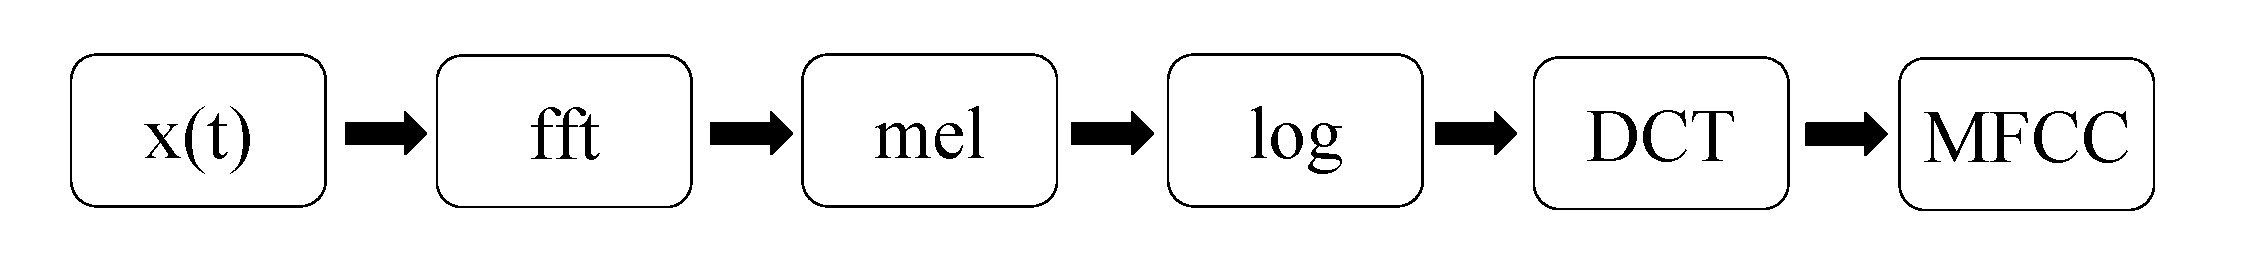
\includegraphics[width = 0.7\textwidth]{./figures/autres/schema_MFCC.pdf}
%%\caption{Schéma de la conception des MFCC}
%%\label{fig:schema_mfcc}
%%\end{figure}
%
%L'échelle Mel est une échelle de hauteur de sons issus de la psycho-acoustique. Son échelle est construite afin qu'un doublement de mel corresponde à un doublement de la fréquence perçu. Par exemple pour un son pur à 1000 Hz (correspondant à 1000 mel), le son perçu deux fois plus aigu sera un son à environ 3428 Hz et non à 2000 Hz. L'échelle des Mel est alors définit par la relation \ref{eq:melScale} permettant ainsi de conserver le rapport 2 entre les deux sons (le signal à 3428 Hz est alors à 2000 mel),
%
%\begin{equation}\label{eq:melScale}
%mel = 1127 \ln\left(1+\frac{f}{700}\right).
%\end{equation}
%
%
%\item \textbf{paramètres harmoniques} : Cette catégorie regroupe des descripteurs comme la détermination de la fréquence fondamental, de  l'inharmonicité ou bien du tristimulus du signal.
%
%\item \textbf{paramètres perceptifs} : Cette dernière classe regroupe les indicateurs psycho-acoustique comme l'acuité ou la sonie du signal.\\
%\end{itemize}
%
%Dans son article, Peeters \cite{Peeters} résume un ensemble de descripteurs couramment utilisés dans le domaine de la reconnaissance de parole \cite{Kim} ou le domaine de la musique \cite{Fu} qui sont ceux qui sont également utilisés pour des ambiances sonores environnementales \cite{Cowling}, \cite{Haddad}, \cite{Defreville}.


%
%En raison de l'utilisation de l'échelle Mel, les MFCC sont le plus souvent utilisés dans le cas de la détection de signaux de paroles \cite{Wu}.

%\subsection{Analyse en Composante Principale}\label{part:ACP}
%
%L'utilisation de plusieurs descripteurs génèrent un ensemble de données décrivant chaque signal spécifiquement.
%
%\begin{equation}
%\mathbf{X} =
%\begin{pmatrix}
%x_{11}& x_{12} & \dots & x_{1p} \\
%x_{21}& x_{22} & \dots & x_{2p} \\
%\vdots & \vdots & \ddots & \vdots \\
%x_{N1}& x_{N2} & \dots & x_{Np}
%\end{pmatrix}
%\end{equation}
%
%où $N$ est le nombre de signaux traités et $p$ le nombre de variable utilisé pour les décrire. Néanmoins, leur représentation graphique en un nuage de point qui permettrait de visualiser la corrélation entre les signaux n'est pas facile au delà de $p = 3$ car la dimension de problème n'est alors plus représentable. De plus, certains paramètres sont parfois redondant et ajoute une dimension aux problème rendant la représentations des corrélations entre elles plus difficile. \\
%
%L'Analyse en Composante Principale (ACP) se propose alors de réduire les dimensions du problème en passant d'un espace à $p$ dimensions à un sous-espace réduit $k$ (le plus généralement $k = 2$ ou $k=3$). Ces nouvelles variables $k$ sont construites à partir de combinaisons linéaire des $p$ variables initiales et celle qui présentent les plus fortes variances. Elles sont appelées \og composante principale \fg{} et forment de nouveaux axes de représentations appelé \og axes principaux \fg{}. Ce choix permet de conserver le plus d'information possible. Pour cela le sous-espace est construit afin que sa distance avec les données de $\textbf{X}$ soit minimale et que la projection du nuage de points est une dispersion (ou inertie) maximale.
%
%L'extraction de paramètres des signaux permet alors d'apporter de nouvelles informations qui vont permettre ainsi de séparer les signaux en fonction des classes de son présentes. Leur choix doit permettre de rendre chaque description des classe unique afin que la classification soit réussie.

%\subsection{Classificateurs}\label{part:classificateur}
%
%L'étape de classification vise à reconnaitre les différentes classes de sons présentes à l'aide des descripteurs offrant ainsi une référence qui permettra la reconnaissance des sources lors de la phase de test. Les méthodes de classification peuvent être considéré par deux approches : discriminative ou générative.\\
%
%La première approche modélisent directement la règle de classification. Les plus populaires sont les \og $k$-plus-proches voisins \fg{} ($k$-NN pour \textit{k-Nearest-Neighbours} en anglais) ou les Vecteurs à Support de Machine (SVM pour \textit{Support Machine Vectors} en anglais). \\
%
%La méthode $\mathbf{k-}$\textbf{NN} consiste à calculer les distances entre un échantillon testé $x$ et les données issus de l'apprentissage. La classe ayant alors les $k$ distances les plus faibles est donc celle de l'échantillon $x$.\\
%
%La méthode \textbf{SVM}, quant à elle, consiste à déterminer un séparateur linéaire entre deux ensembles de telle façon que la distance normal des plus proches échantillons des classes à cette courbe soit maximisée. Cette courbe est appelé \textit{hyperplan} et les échantillons qui maximisent la distance sont les \textit{vecteurs supports}. Dans le cas où le problème ne possède pas d'hyperplan linéaire, l'espace de représentation des données est modifié, pouvant jusqu'à être défini dans un espace à dimension infini, afin d'en obtenir un.\\
%
%Les méthodes génératrices visent à modifier la distribution des données $x$ pour ensuite réaliser la classification. Les plus utilisés sont les Modèles de Mixtures Gaussiens (abrégé GMM pour \textit{Gaussian Mixture Models} en anglais) et le Modèle de Markov Caché (HMM pour \textit{Hidden Markov Model}).\\
%
%Un modèle de mélanges gaussiens modélise une distribution de données comme une somme de gaussiennes pondérées (équation \ref{eq:GMM}).
%
%\begin{equation}\label{eq:GMM}
%g(x,\bm{\mu},\bm{\sigma}) = \sum_{n = 1}^N \pi_n f(x,\bm{\mu}, \bm{\sigma})
%\end{equation}
%
%avec pour distribution gaussienne
%
%\begin{equation}
%f(x,\mu, \sigma) = \frac{1}{\sigma \sqrt{2\pi}}e^{\frac{(x-\mu)^2}{2\sigma^2}}
%\end{equation}
%
%%\begin{figure}[hbtp]
%%\centering
%%\includegraphics[scale=0.35]{../../../../Pictures/GMM.pdf}
%%\caption{GMM (n trait plein) composé de deux distributions gaussiennes ($\bm{\pi} = \left[ 0.35,  0.75 \right]$, $\bm{\mu} = \left[9,  15.8 \right]$, $\bm{\sigma} = \left[ 3.2,  4.3 \right]$) pour $x \in \left[0~25 \right]$ }
%%\end{figure}
%
%
%C'est par l'algorithme de \textit{Esperance-Maximisation} \cite{Dempster} que les paramètres optimaux (moyenne $\bm{\mu}$, variance $\bm{\sigma}$, amplitude $\bm{\pi}$) sont trouvés. Le principe consiste à augmenter la probabilité entre le modèle et les données de manière itérative en effectuant deux phases de calculs distinctes :
%\begin{itemize}
%\item \og Espérance \fg{}, on estime des données inconnues, sachant les données observées ($x$) et la valeur des paramètres déterminée à l'itération précédente (moyenne et écart type dans le cas de distribution gaussienne).
%\item \og Maximisation \fg, on met à jours les paramètres en maximisant la vraisemblance de l'estimation des données et du modèle gaussien.\\
%\end{itemize}
%
%Cette étape de maximisation fait intervenir la règle d'inversion de Bayes (\ref{eq:Bayes}).
%
%\begin{equation}\label{eq:Bayes}
%P(y \in g_n \vert y) = \frac{P(y \vert y \in g_n)P(y \in g_n)}{P(y)}
%\end{equation}
%
%avec
%\begin{itemize}
%\item $P(y \vert y \in g_n)$, la densité de probabilité de la classe $g_n$,
%\item $P(y \in g_n)$, la densité de probabilité de $y$,
%\item $P(y)$, la densité de probabilité de $y$ ($P(y) = 1$).\\
%\end{itemize}
%
%Lors de la phase de test, la classe $g_n$ dans laquelle l'élément testé $y$ a le plus de chance d'appartenir est déterminé en maximisant la probabilité à postériori $P(y\in g_n\vert y)$ (\ref{eq:maxArg}).
%
%\begin{equation}\label{eq:maxArg}
%f(y,\mu, \sigma) = \text{arg max } P(y\in g_n\vert y)
%\end{equation}
%
%Dans le cadre d'un GMM, (\ref{eq:Bayes}) devient
%\begin{equation}
%P(y \in g_n) = \frac{\pi_n f(y,\mu,\sigma)}{\sum_{l = 1}^N \pi_l f(y,\mu, \sigma)}
%\end{equation}
%
%Une autre technique de classification couramment utilisé est le Modèle de Markov Caché \cite{Rabiner}. Le principe générale est de déterminer la succession la plus probable d'évènement à partir d'observations faites.\\
%Cette méthode se base sur les chaines de Markov qui décrit l'état d'un processus stochastique à l'instant $t$ en fonction seulement de son état à l'instant $t-1$ avec la probabilité de passer d'un état $i$ à un état $j$ qui ne varie pas avec le temps.\\
%
%Dans le cadre d'un modèle de Markov caché, l'état du système n'est pas disponible mais seulement des observations correspondant à l'état du processus. Le modèle dépend alors de 5 paramètres :
%
%\begin{itemize}
%\item $S$, l'ensemble des états possibles,
%\item $A$, l'ensemble des observations émis par les états,
%\item $\Pi$, la loi de probabilité à l'état initial,
%\item $T$, a matrice des probabilités de transitions d'un état à un autre.
%\item $E$, la matrice de probabilité des observations pour chaque état.\\
%\end{itemize}
%
%C'est durant la phase d'apprentissage que l'ensemble de ces paramètres du modèle caché sont déterminé par la maximisation de vraisemblance (algorithme d'\textit{Espérance-Maximisation}). Chaque classe de son est alors caractérisé par un ensemble de paramètre. La phase de test cherche ensuite à maximiser la \textit{log}-vraisemblance (Maximum a Posteriori) entre les paramètres de l'échantillon testé et ceux issus de l'apprentissage.
%
%Si ces techniques permettent d'identifier une source sonore, ce ne sont pas des outils adapté pour des mixtures sonores urbaines composée d'une multitude de sources très variés : trafic d'une voiture, d'un avion, bruit de pas, klaxon, oiseaux, musique... Ces sons ont des variations temporelles et fréquentielles très différentes. Pour cela, les techniques de séparations de sources semblent plus adaptés à ces ambiances sonores.
%
%\subsection{Applications}
%
%Ces méthodes de classification et de reconnaissance sont utilisée dans de nombreux domaines économique \cite{Hu}, médicale (\cite{Yu}, \cite{Gorriz}) ou de l'imagerie \cite{}.
%
%
%Dans le cadre de signaux audiophoniques, les
%
%Dans le cadre de la musique, ces techniques visent notamment à classer les musiques par genre, artistes ou époques (\cite{Tzanetakis}, \cite{Panagakis}, \cite{Berenzweig},\cite{Ellis}, \cite{Heitolla}). Ces outils trouvent leur intérêt dans l'utilisation et l'écoute de contenu musicaux sur internet (site de streaming par exemple) de plus en plus massive qui nécessite d'avoir des outils automatique de description des enregistrements audio afin de les classer mais aussi afin de suggérer à l'auditeur des contenus similaire qu'il pourrait aimer.  Les outils de séparation sont, quant à eux, notamment utile dans la restauration de vieux enregistrements.
%
%Cowling, Haddad, Defréville...
%Problème du recouvrement des sources sonores dans un milieu urbain
%
%Delgado \& al. \cite{Delgado} se sont eux intéressé à ajouter un étape intermédiaire consistant à réduire le nombre de paramètres et donc le temps de calcul. Leur étude s'intéressait à l'identification d'environnement sonore varié (rue, restaurant, casino, train ...) en vue de développer cet algorithme sur des smartphones.\\
%
%\subsection{Réseaux de Neurones Artificiels}
%\bibliographystyle{unsrt}
%\bibliography{../bibliographie}

%\end{document}
